\chapter{Formal Concept Analysis}
\label{chapter:formal-concept-analysis}

\FCA (FCA) \cite{Wille_Restructuring,WILLE1992493,ganter1999formal} is an approach to reasoning about \textit{concepts} and
corresponding \textit{conceptual structures} in terms of lattice theory and sets. It was first proposed by Wille in his monograph
\textit{Restructuring Lattice Theory} \cite{Wille_Restructuring}, which was an attempt to reestablish a connection between
the theory and practice of lattices.

A core aspect of FCA’s foundation is the mathematisation of the philosophical view of concepts, in which a they are
understood as a unit comprising two parts: the \textit{extension}, which is the collection of things said to be instances
of the concept, and the \textit{intension}, which contains those properties used to ascribe meaning to the concept
\cite{DUQUENNE1999407}.

\section{Basic Notions in Formal Concept Analysis}
\label{section:basic-notions}

Without any formal introduction to this this topic, one can readily grasp the concept of a `person'. We can point to many
sense-making properties of this concept: \textit{mortal}, \textit{warm-blooded}, \textit{mammalian}, and so on. Listing some
of the instances included in the extension of this concept is not particularly challenging either---for example, \textit{the
author of this work}, or \textit{the reader}. What is also clear is that exhaustively specifying a list of either the
intension or extension is likely to be a challenging task, even when these lists are finite, although finiteness need
not be a property.

This leads us to what is usually the starting point of FCA a structure called a \textit{formal context}, or simply a
context. A context restricts our ontological consideration to a reduced universe of discourse, as well as detailing the
underlying structural relationship that exists between elements in this universe \cite{Wille_Restructuring,Dau2005}.

\begin{definition}
	\index{formal context} \label{definition:formal-context} A formal context $\context = \GMI$ is a triple comprised of a
	set $G$ of objects , a set $M$ of attributes, and a binary relation $I \subseteq G \times M$ referred to as an `incidence'
	relation. For an object-attribute pair $(g,m) \in I$ we may say \say{The object $g$ \textit{has} the attribute $m$}.
\end{definition}

We consider the set of objects $G$ (from the German \textit{Gegenstände}) as the extensional dimension of the context, whereas
the set of attributes $M$ (from the German \textit{Merkmale}) represents the intensional dimension. However, the
distinction between the extensional and intensional dimensions of the context is largely a matter of convention, or when
introducing a FCA a means of improving intuition. There is no strict requirement around what these sets are made up of, or
even that they be distinct, and so it is perfectly acceptable to have a context where the objects and attributes are the
same set; for example, the context $(\mathbb{N}, \mathbb{N}, \texttt{divides })$ which describes the division
relationship between natural numbers.

It should be noted that, while the presence of an object--attribute pair $(g,m)$ in the incidence relation is
interpreted as the object satisfying the respective attribute, FCA is concerned only with \textit{positive} information,
and so the absence of a pair in the relation is not usually interpreted to mean that the object has the negation of the attribute.
We will discuss, in more depth, the rather troubling matter of negation and negative attributes in
\Cref{section:attribute-logic}.

When the cardinalities of $G$ and $M$ are small, contexts may be represented as a cross-table such as in \Cref{cxt:grouplikes}.
Each object is represented by a row in the table, each attribute by a column, and each pair in the incidence relation is
marked with an `$\times$' at the appropriate position \cite{ganter1999formal}. Given a context presented in this form,
it is a trivial task to identify all the attributes that a particular object satisfies: One need only scan across the respective
row and note where the marks appear. The resulting set of attributes is called the \textit{object's intent}. The dual
notion of an \textit{attribute extent} can be found by traversing down a column in the table.

\begin{figure}[H]
	\centering
	\small
	\begin{cxt}
		\label{cxt:grouplikes} \cxtName{\textbf{\texttt{Algebraic Structures}}} \att{\texttt{closure}} \att{\texttt{associativity}}
		\att{\texttt{identity}} \att{\texttt{inverse}} \att{\texttt{commutativity}} \obj{x....}{\texttt{magma}} \obj{xx...}{\texttt{semigroup}}
		\obj{xxx..}{\texttt{monoid}} \obj{xxxx.}{\texttt{group}} \obj{xxxxx}{\texttt{abelian group}} \obj{x.xx.}{\texttt{loop}}
		\obj{x..x.}{\texttt{quasigroup}} \obj{.xxx.}{\texttt{groupoid}} \obj{.xx..}{\texttt{category}} \obj{.x...}{\texttt{semicategory}}
	\end{cxt}
	\caption{A formal context showing necessary properties of group-like structures.}
	\label{context:formal-context-group-structures}
\end{figure}

Using this approach, we can see that the intent of $\texttt{magma}$ is the singleton $\{\texttt{closure}\}$, while the
extent of \texttt{closure} is the set $\{\texttt{magma,semigroup,monoid,group,ableian group,loop,quasigroup}\}$.

This approach to determining object extents and attribute intents becomes impractical when considering non-trivial contexts,
or large sets of objects and attributes. The procedure can be formally described by the \textit{derivation operators}:
% \footnote{It is common to denote
% either derivation operator with a prime and use the surrounding context to resolve ambiguity, so $A^{\uparrow}$ and $B^{\downarrow}$ would become
% $A'$ and $B'$, respectively. We avoid this notation as later on it will become increasingly challenging to avoid ambiguity while maintaining
% pleasing notation. In cases where a derivation operator is applied to a singleton of objects $\{g\}$ (\textit{resp.} attributes $\{m\}$) we omit
% the parenthesis and write $g^{\uparrow}$ (\textit{resp.} $m^{\downarrow}$)}

\begin{definition}
	\index{derivation operators} \label{definition:derivation-operators} Given a context $\GMI$, the \textit{derivation
	operators} are two maps $(\cdot)^{\uparrow}: \pset{G}\to \pset{M}$ and $(\cdot )^{\downarrow}: \pset{M}\to \pset{G}$.
	Then, for any subsets $A \subseteq G$ and $B \subseteq M$,
	\begin{align*}
		A^{\uparrow}   & \coloneqq \{m \in M \mid \forall g \in A, \; (g,m) \in I\} \\
		B^{\downarrow} & \coloneqq \{g \in G \mid \forall m \in B, \; (g,m) \in I\}
	\end{align*}
\end{definition}

The derivation operators describe a mapping from a subset $A \subseteq G$ of objects in a context to the corresponding subset
of attributes that each (and every) object in $A$ related to. The dual notion holds for starting with a subset of
attributes. As an example, we might wish to determine the set of attributes satisfied by the objects
$\{\texttt{group,groupoid,abelian group}\}$. Application of the $(\cdot)^{\uparrow}$ derivation operator to this set yields
$\{\texttt{associativity,identity,inverse }\}$.

To offer another perspective on the derivation operators, obvserve that the derivation of a set $A\subseteq G$ of
objects is the intersection of each object intent, and so we have
\begin{align*}
	A^{\uparrow}= \bigcap \{a^{\uparrow}\mid a \in A\}     & \qquad A \subseteq G  \\
	B^{\downarrow}= \bigcap \{b^{\downarrow}\mid b \in B\} & \qquad B \subseteq M.
\end{align*}

In fact, we have already explored a more general perspective on the derivation operators in \Cref{section:closure-systems}
through the notion of closure operators and Galois connections. The proposition below recontextualises properties of
Galois connections in the setting of FCA.

\begin{proposition}
	\label{proposition:derivation-operators-galois} Let $\GMI$ be a formal context and consider the subsets $X,X_{1}\subseteq
	G$ of objects (\textit{resp.} $Y,Y_{1}\subseteq M$ of attributes) then
	\begin{align}
		 & X \subseteq X_{1}\Rightarrow X_{1}^{\uparrow}\subseteq X^{\uparrow} & \textit{(resp.)}         & \qquad Y \subseteq Y_{1}\Rightarrow Y_{1}^{\downarrow}\subseteq Y^{\downarrow}\label{equation:galois-1} \\
		 & X \subseteq X^{\uparrow \downarrow}                                 & \textit{(resp.)}         & \qquad Y \subseteq Y^{\downarrow \uparrow}\label{equation:galois-2}                                     \\
		 & X^{\uparrow}= X^{\uparrow \downarrow \uparrow}                      & \textit{(resp.)}         & \qquad Y^{\downarrow}= Y^{\downarrow \uparrow \downarrow}\label{equation:galois-3}                      \\
		 & X \subseteq Y^{\downarrow}\tiff X^{\uparrow}\supseteq Y             & \label{equation:galois-4}
	\end{align}
\end{proposition}

If we consider the powerset lattices of $\pset{G}$ and $\pset{M}$ under their usual inclusion orders, then the
derivation operators constitute a Galois connection on these sets: \Cref{equation:galois-1,equation:galois-2,equation:galois-3}
are just a rephrasing of \Cref{equation:ord_galois-1,equation:ord-galois-2,equation:ord-galois-3}; while
\Cref{equation:galois-4} rephrases \Cref{proposition:fundamental-galois}. Mirroring the `discussion' on Galois connections,
we obtain the closure systems $\mathcal{G}$ and $\mathcal{M}$ on $G$ and $M$, respectively. Each of these closure
systems form a complete lattice where, recounting \Cref{theorem:closure-systems-lattices}, meets and joins are given by:
%
\begin{align*}
	 & \underset{i \in I}\bigwedge A_{i}= \underset{i \in I}\bigcap A_{i}\quad \text{ and }\quad \underset{i \in I}\bigvee A_{i}= \big(\underset{i \in I}\bigcup A_{i}\big)^{\uparrow \downarrow} & \quad A\subseteq \mathcal{G} \\
	 & \underset{i \in I}\bigwedge B_{i}= \underset{i \in I}\bigcap B_{i}\quad \text{ and }\quad\underset{i \in I}\bigvee B_{i}= \big( \underset{i \in I}\bigcup B_{i}\big)^{\downarrow \uparrow} & \quad B\subseteq \mathcal{M}
\end{align*}

We recall the discussion at the end of \Cref{subsection:galois-connections} where it was shown that a pair of mappings
that form a Galois connection are dually isomorphic when their domains are restricted to the associated closure systems.
With the aid of \Cref{figure:two-lattices}, we note this correspondence between the lattices of closure systems
$\mathcal{G}$ and $\mathcal{M}$.

\vspace{-5em}
\begin{figure}[H]
	\centering
	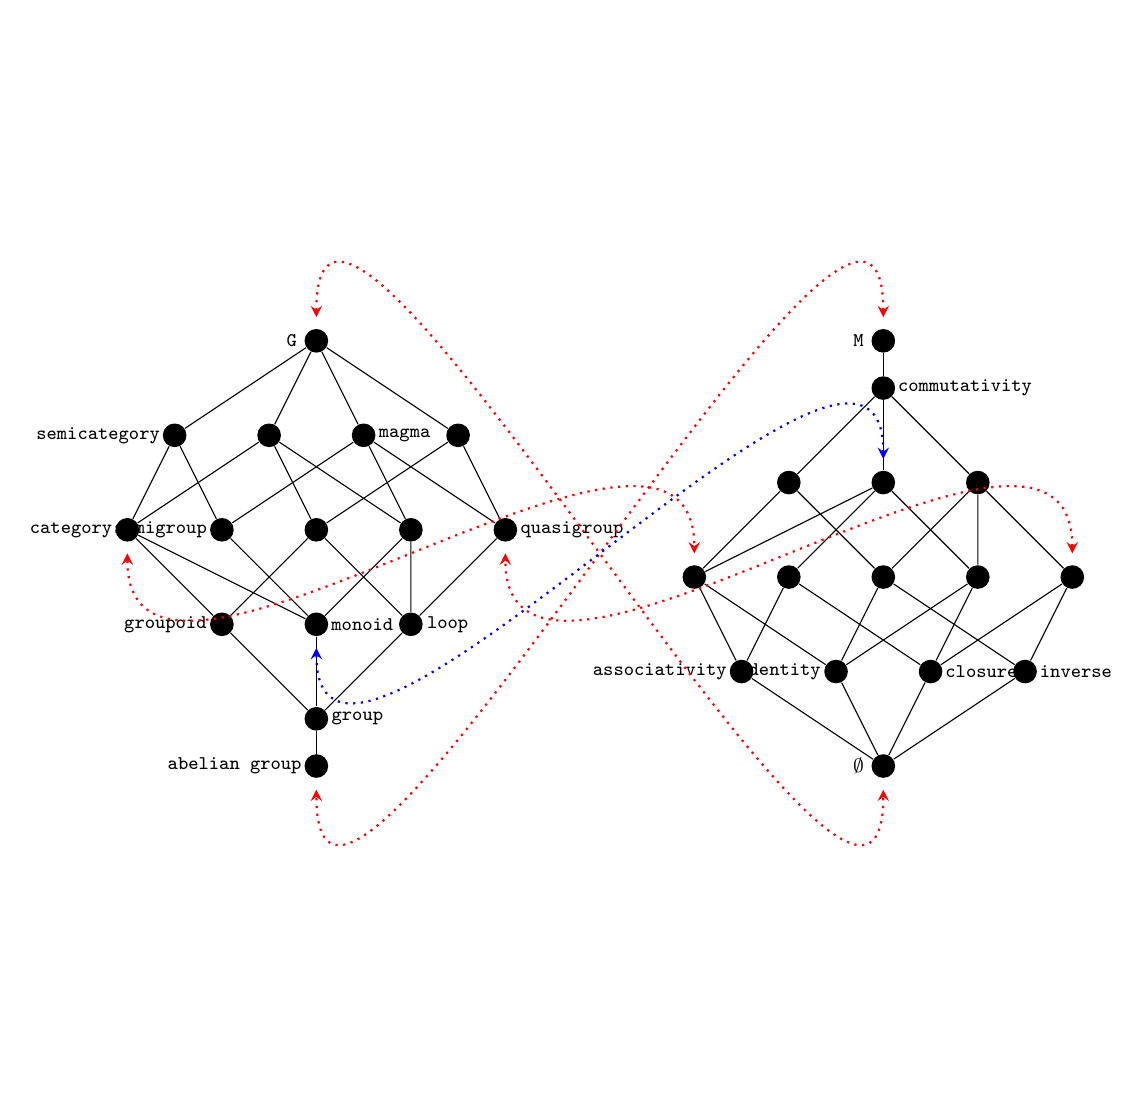
\begin{tikzpicture}[scale=0.6, every node/.style={circle, fill=black, inner sep=0.5pt, minimum size=3mm}]
		\node (a1) at (0,4) [label=left:{\scriptsize \texttt{G}}] {};

		\node (b1) at (-3,2) [label=left:{\scriptsize \texttt{semicategory}}] {};
		\draw (a1) -- (b1);

		\node (b2) at (-1,2) [label=left:{\scriptsize \texttt{}}] {};
		\draw (a1) -- (b2);

		\node (b3) at (1,2) [label=right:{\scriptsize \texttt{magma}}] {};
		\draw (a1) -- (b3);

		\node (b4) at (3,2) [label=right:{\scriptsize \texttt{}}] {};
		\draw (a1) -- (b4);

		\node (c1) at (-4,0) [label=left:{\scriptsize \texttt{category}}] {};
		\draw (c1) -- (b1);
		\draw (c1) -- (b2);

		\node (c2) at (-2,0) [label=left:{\scriptsize \texttt{semigroup}}] {};
		\draw (c2) -- (b1);
		\draw (c2) -- (b3);

		\node (c3) at (0,0) [label=left:{\scriptsize \texttt{}}] {};
		\draw (c3) -- (b2);
		\draw (c3) -- (b4);

		\node (c4) at (2,0) [label=right:{\scriptsize \texttt{}}] {};
		\draw (c4) -- (b2);
		\draw (c4) -- (b3);

		\node (c5) at (4,0) [label=right:{\scriptsize \texttt{quasigroup}}] {};
		\draw (c5) -- (b3);
		\draw (c5) -- (b4);

		\node (d1) at (-2,-2) [label=left:{\scriptsize \texttt{groupoid}}] {};
		\draw (d1) -- (c1);
		\draw (d1) -- (c3);

		\node (d2) at (0,-2) [label=right:{\scriptsize \texttt{monoid}}] {};
		\draw (d2) -- (c1);
		\draw (d2) -- (c2);
		\draw (d2) -- (c4);

		\node (d3) at (2,-2) [label=right:{\scriptsize \texttt{loop}}] {};
		\draw (d3) -- (c3);
		\draw (d3) -- (c4);
		\draw (d3) -- (c5);

		\node (e1) at (0,-4) [label=right:{\scriptsize \texttt{group}}] {};
		\draw (e1) -- (d1);
		\draw (e1) -- (d2);
		\draw (e1) -- (d3);

		\node (f1) at (0,-5) [label=left:{\scriptsize \texttt{abelian group}}] {};
		\draw (f1) -- (e1);

		\begin{scope}[shift={(12,0)}]
			\node (ra1) at (0,-5) [label=left:{\scriptsize $\emptyset$}] {};

			\node (rb1) at (-3,-3) [label=left:{\scriptsize \texttt{associativity}}] {};
			\draw (ra1) -- (rb1);

			\node (rb2) at (-1,-3) [label=left:{\scriptsize \texttt{identity}}] {};
			\draw (ra1) -- (rb2);

			\node (rb3) at (1,-3) [label=right:{\scriptsize \texttt{closure}}] {};
			\draw (ra1) -- (rb3);

			\node (rb4) at (3,-3) [label=right:{\scriptsize \texttt{inverse}}] {};
			\draw (ra1) -- (rb4);

			\node (rc1) at (-4,-1) [label=left:{\scriptsize \texttt{}}] {};
			\draw (rc1) -- (rb1);
			\draw (rc1) -- (rb2);

			\node (rc2) at (-2,-1) [label=left:{\scriptsize \texttt{}}] {};
			\draw (rc2) -- (rb1);
			\draw (rc2) -- (rb3);

			\node (rc3) at (0,-1) [label=left:{\scriptsize \texttt{}}] {};
			\draw (rc3) -- (rb2);
			\draw (rc3) -- (rb4);

			\node (rc4) at (2,-1) [label=right:{\scriptsize \texttt{}}] {};
			\draw (rc4) -- (rb2);
			\draw (rc4) -- (rb3);

			\node (rc5) at (4,-1) [label=right:{\scriptsize \texttt{}}] {};
			\draw (rc5) -- (rb3);
			\draw (rc5) -- (rb4);

			\node (rd1) at (-2,1) [label=left:{\scriptsize \texttt{}}] {};
			\draw (rd1) -- (rc1);
			\draw (rd1) -- (rc3);

			\node (rd2) at (0,1) [label=right:{\scriptsize \texttt{}}] {};
			\draw (rd2) -- (rc1);
			\draw (rd2) -- (rc2);
			\draw (rd2) -- (rc4);

			\node (rd3) at (2,1) [label=right:{\scriptsize \texttt{}}] {};
			\draw (rd3) -- (rc3);
			\draw (rd3) -- (rc4);
			\draw (rd3) -- (rc5);

			\node (re1) at (0,3) [label=right:{\scriptsize \texttt{commutativity}}] {};
			\draw (re1) -- (rd1);
			\draw (re1) -- (rd2);
			\draw (re1) -- (rd3);

			\node (rf1) at (0,4) [label=left:{\scriptsize \texttt{M}}] {};
			\draw (rf1) -- (re1);
		\end{scope}
		\draw[red, dotted, stealth-stealth, line width=0.8pt] (12,4.5) to[out=90, in=270] (0,-5.5);
		\draw[red, dotted, stealth-stealth, line width=0.8pt] (16,-0.5) to[out=90, in=270] (4,-0.5);
		\draw[red, dotted, stealth-stealth, line width=0.8pt] (-4,-0.5) to[out=270, in=90] (8,-0.5);
		\draw[red, dotted, stealth-stealth, line width=0.8pt] (0,4.5) to[out=90, in=270] (12,-5.5);
		\draw[blue, dotted, stealth-stealth, line width=0.8pt] (0,-2.5) to[out=270, in=90] (12,1.5);
	\end{tikzpicture}
	\vspace{-6em}
	\caption{The lattices induced by the closure systems $\mathcal{G}$ and $\mathcal{M}$. \textcolor{red}{Each node in a
	lattice represents the set comrpising of all labels reachable from below}}
	\label{figure:two-lattices}
\end{figure}

Earlier, it was suggested that Galois connections are particularly interesting when the closure systems they induce are
themselves interesting, and, future discussion of an example of such interesting closure systems was promised. Let us now
give such an example, and in doing so provide some intution for why Galois connections are a useful way of modelling
concepts, to be introduced immediately afterwards.

Consider the concept derived from the algebraic structure of a \textit{monoid}: a set equipped with a binary operation that
satisfies the properties of closure, associativity, and that has an identity element. We should want to include in the
extension of this concept all those algebraic structures that would be considered subclasses of monoids. These are those
structures which satisfy the properties of a monoid (and possibly additional properties). Of course, a \textit{monoid}
should be a member of this extension. Another structure we should expect to see in this extension is that of a \textit{group},
which satisfies the requirements while also having the property of invertibility.

Now let us consider the concept derived from a \textit{group}. We have just shown that a group is a subclass of monoid,
so it should follow that the extension of a group must be a subset of the extension of a monoid. What of the intension?
Suppose the intension of the concept of a monoid were not a subset of that of a group, then monoids would have to satisfy
some property that groups did not. This creates a contradiction, as it would mean we could not properly consider a group
to be a subclass of a monoid.

This reveals the relationship between concepts, such that when we move from the more general concept (monoid) to the
more specific concept (group), the extension becomes smaller while the intension grows. The extension of group is
contained within the extension of monoid, but the intension of monoid is contained within the intension of group. This
inverse relationship between the extensions and intensions of concepts is precisely the kind of relationship described
by a Galois connection.

With this in mind, it is finally an appropriate time to define what is meant by \textit{formal concept}:

\begin{definition}
	\index{formal concept} \index{lattice! concept lattice} \label{definition:formal-concept} A \emph{formal concept} of a
	context $\GMI$ is a pair $(A,B)$ where $A \subseteq G$ and $B\subseteq M$ where $A^{\uparrow}= B$ and
	$B^{\downarrow}= A$. We call $A$ the \emph{concept extent} and $B$ the \emph{concept intent}. We write $\BGMI$ to
	denote the set of all concepts of $\GMI$.
\end{definition}

A concept is then a pair of closed sets, where each set represents either the extensional or intensional perspective on
the concept. Indeed, the extension and intension are related by virtue of being the inverses of one another under the
derivation operators, and so there is a degree of redundancy in this definition since knowing the concept extension is sufficient
to learning the concept intension and vice verse \cite{ganter2016conceptual}. Yet, we persevere with this redundancy as it
offers a unifying perspective.

One pleasing consequence of the definition of a formal concept is that, for any set $A\subseteq G$ of objects, the set $A
^{\uparrow}$ will always be a concept intent, and facilitates the construction of
$(A^{\uparrow \downarrow}, A^{\uparrow})$ which is similarly always a concept; in general, the set $A$ is a concept
extent if it is equal to its' closure $A^{\uparrow \downarrow}$. The dual perspective holds, and so for a set $B \subseteq
M$ of attributes, $B^{\downarrow}$ is always a concept extent. We are even more fortunate in that we have already extensively
discussed the collection(s) of closed sets of objects and attributes and what structure they might have: of course,
these are the closure systems $\mathcal{G}$ and $\mathcal{M}$ and their corresponding lattice structure.

To make this idea concrete, we reconsider the previous discussion where we (informally) described the concept of a monoid.
It follows that the derivation $\{\texttt{monoid }\}^{\uparrow}$ yields the intent
\[
	\{\texttt{closure,associativity,identity}\}.
\]
%
In turn, the derivation of the concept intent results in the set
\[
	\{\texttt{monoid,group,abelian group}\},
\]which is the concept extent, and so
\[
	\big(\{\texttt{monoid,group,abelian group}\}, \{\texttt{closure,associativity,identity }\}\big)
\]
is a formal concept of \Cref{cxt:grouplikes}.

The union of concept extents (intents) is not guaranteed to yield another concept extent (intent), whereas the
intersection of concept extents (intents) will always result in another concept extent (intent). That is to say, the
closure systems $\mathcal{G}$ and $\mathcal{M}$ are not closed under taking arbitrary unions, while they are under arbitrary
intersections.

\begin{proposition}
	\label{proposition:intersection-union-concepts} Let $T$ be an indexing set, then for every $t \in T$
	$A_{t}\subseteq G$ is a set of objects, then
	\[
		\big( \underset{t \in T}\bigcup A_{t}\big)^{\uparrow}= \underset{t \in T}\bigcap A_{t}^{\uparrow}
	\]
\end{proposition}

If we examine the lattices in \Cref{figure:two-lattices}, we observe that the two derivation operators map to and from the
concept intent and extent (shown by the dotted blue arrows). This observation suggests a more consolidated perspective: The
two lattices can be unified into a single structure where elements of the lattice are precisely the pairs $(A,B)$ where $A
\in \mathcal{G}$ and $B \in \mathcal{M}$ and also $A^{\uparrow}= B$ and $B^{\downarrow}= A$. In other words, the lattice
of concepts. We appropriately call this structure the \textit{concept lattice} of a formal context, and write $\CLGMI$
to refer to the set of all concepts equipped with this structure.

\begin{figure}[H]
	\centering
	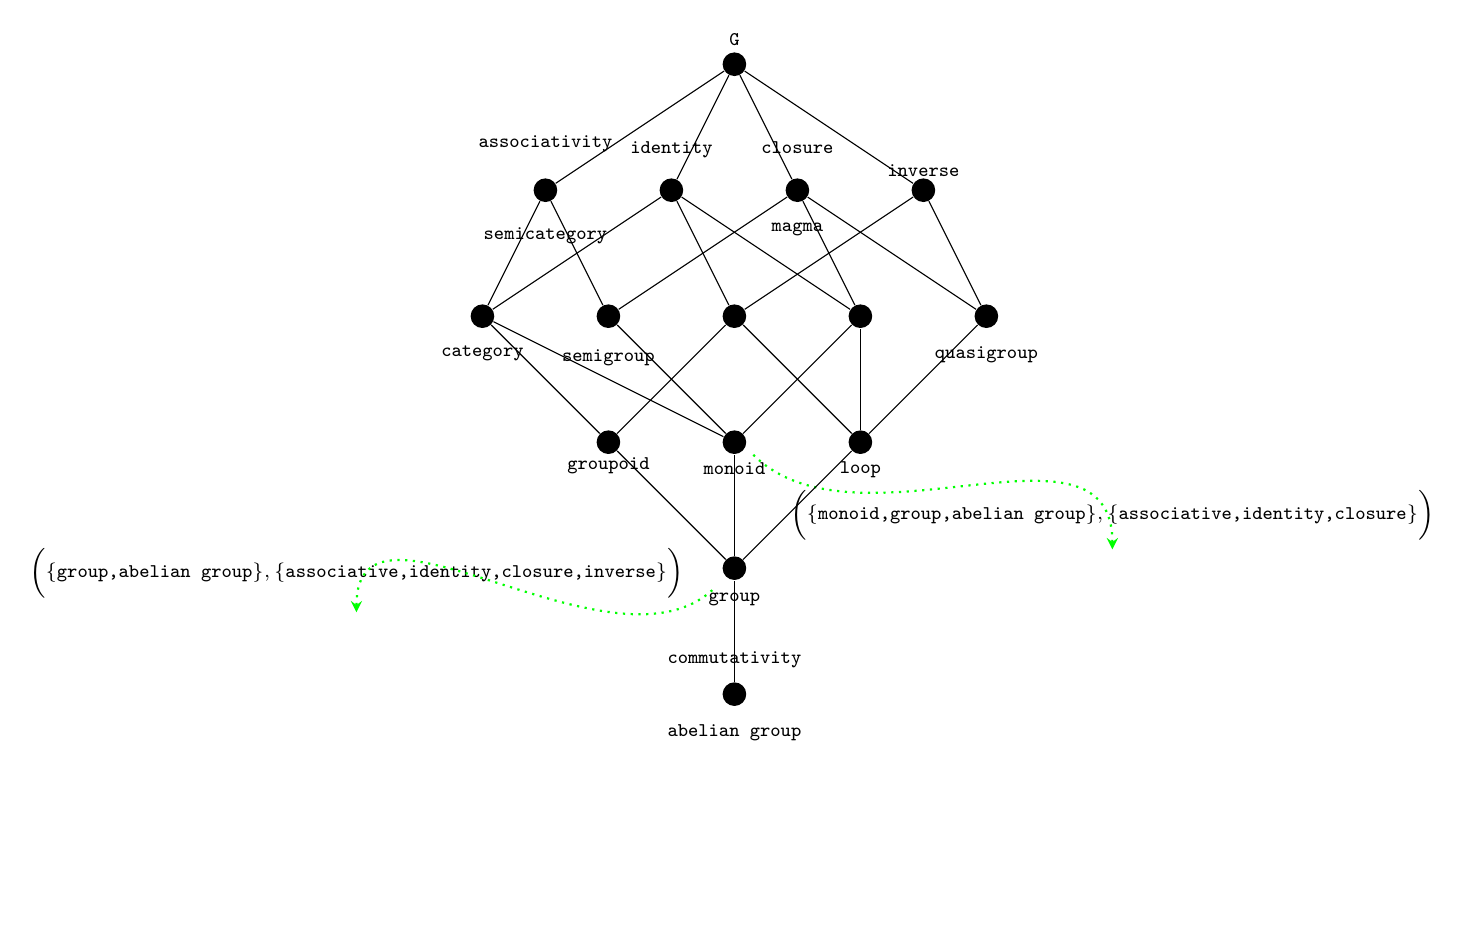
\begin{tikzpicture}[scale=0.8, every node/.style={circle,fill=black,inner sep=0.5pt,minimum size=3mm}]
		%––––– row 1 –––––
		\node (a1) at (0,4) [label={[anchor=south,yshift=0mm]above:{\scriptsize\texttt{G}}}] {};

		%––––– row 2 –––––
		\node (b1)
			at
			(-3,2)
			[
				label={[anchor=south,yshift=-4.5mm]above:{\scriptsize\texttt{associativity}}},
				label={[anchor=north,yshift=4.5mm,text depth=0pt]below:{\scriptsize\strut\texttt{semicategory}}}
			]
			{};
		\draw (a1) -- (b1);

		\node (b2) at (-1,2) [label={[anchor=south,yshift=-2mm]above:{\scriptsize\texttt{identity}}}] {};
		\draw (a1) -- (b2);

		\node (b3)
			at
			(1,2)
			[
				label={[anchor=south,yshift=-1mm]above:{\scriptsize\texttt{closure}}},
				label={[anchor=north,yshift=1mm,text depth=0pt]below:{\scriptsize\strut\texttt{magma}}}
			]
			{};
		\draw (a1) -- (b3);

		\node[fill=none]
			(eg)
			at
			(6,-8)
			[
				label={[anchor=south,yshift=-4mm]above:{\scriptsize $\big(\{\texttt{monoid,group,abelian group}\},\{\texttt{associative,identity,closure}\}\big)$ }}
			]
			{};
		\draw[green, dotted, stealth-, line width=0.8pt] (6,-3.7) to[out=90, in=315] (0.3,-2.2);

		\node[fill=none]
			(eg1)
			at
			(-6,-9)
			[
				label={[anchor=south,yshift=-4mm]above:{\scriptsize $\big(\{\texttt{group,abelian group}\},\{\texttt{associative,identity,closure,inverse}\}\big)$ }}
			]
			{};
		\draw[green, dotted, stealth-, line width=0.8pt] (-6,-4.7) to[out=90, in=225] (-0.3,-4.3);

		\node (b4) at (3,2) [label={[anchor=south,yshift=-4mm]above:{\scriptsize\texttt{inverse}}}] {};
		\draw (a1) -- (b4);

		\node (c1)
			at
			(-4,0)
			[label={[anchor=north,yshift=3mm,text depth=0pt]below:{\scriptsize\strut\texttt{category}}}]
			{};
		\draw (c1) -- (b1);
		\draw (c1) -- (b2);

		\node (c2)
			at
			(-2,0)
			[label={[anchor=north,yshift=3mm,text depth=0pt]below:{\scriptsize\strut\texttt{semigroup}}}]
			{};
		\draw (c2) -- (b1);
		\draw (c2) -- (b3);

		\node (c3) at (0,0) {};
		\draw (c3) -- (b2);
		\draw (c3) -- (b4);

		\node (c4) at (2,0) {};
		\draw (c4) -- (b2);
		\draw (c4) -- (b3);

		\node (c5)
			at
			(4,0)
			[label={[anchor=north,yshift=4mm,text depth=0pt]below:{\scriptsize\strut\texttt{quasigroup}}}]
			{};
		\draw (c5) -- (b3);
		\draw (c5) -- (b4);

		\node (d1) at (-2,-2) [label={[anchor=south,yshift=-7mm]below:{\scriptsize\texttt{groupoid}}}] {};
		\draw (d1) -- (c1);
		\draw (d1) -- (c3);

		\node (d2) at (0,-2) [label={[anchor=south,yshift=-6mm]below:{\scriptsize\texttt{monoid}}}] {};
		\draw (d2) -- (c1);
		\draw (d2) -- (c2);
		\draw (d2) -- (c4);

		\node (d3) at (2,-2) [label={[anchor=south,yshift=-5mm]below:{\scriptsize\texttt{loop}}}] {};
		\draw (d3) -- (c3);
		\draw (d3) -- (c4);
		\draw (d3) -- (c5);

		\node (e1) at (0,-4) [label={[anchor=south,yshift=-6mm]below:{\scriptsize\texttt{group}}}] {};
		\draw (e1) -- (d1);
		\draw (e1) -- (d2);
		\draw (e1) -- (d3);

		\node (f1)
			at
			(0,-6)
			[
				label={[anchor=south,yshift=-6mm]above:{\scriptsize\texttt{commutativity}}},
				label={[anchor=north,yshift=6mm,text depth=0pt]below:{\scriptsize\strut\texttt{abelian group}}}
			]
			{};
		\draw (f1) -- (e1);
	\end{tikzpicture}
	\vspace{-6em}
	\caption{The concept lattice corresponding to \Cref{cxt:grouplikes}}
	\label{figure:concept-lattice-group-likes}
\end{figure}

\begin{remark}
	Reading a concept lattice requires a small amount of getting used to: The labels above a node in the diagram
	correspond to attributes, while objects are labelled below a node. Each node represents a concept $C \in \BGMI$. The extension
	of $C$ contains all objects attached to nodes which have a (strictly) downwards path from $C$, while the intension of
	$C$ contains those attributes labelled at nodes where there is a strictly upwards path from $C$.
\end{remark}

The concept lattice is isomorphic to the closure system $\mathcal{G}$ of objects, and dually isomorphic to the closure system
$\mathcal{M}$ of attributes. We now consider the first part of the fundamental result in FCA.

\begin{theorem}[The Basic Theorem of Concept Lattices: Part one]
	\label{theorem:basic-theorem-part1} The concept lattice $\CLGMI$ of a formal context is a complete lattice in which meets
	and joins are given by
	\begin{align*}
		 & \underset{t \in T}\bigwedge (A_{t}, B_{t}) = \Big( \underset{t \in T}\bigcap A_{t}, \; \big(\underset{t \in T}\bigcup B_{t}\big)^{\downarrow \uparrow}\Big) \\
		 & \underset{t \in T}\bigvee (A_{t}, B_{t}) = \Big( \big(\underset{t \in T}\bigcup A_{t}\big)^{\uparrow \downarrow},\; \underset{t \in T}\bigcap B_{t}\Big)
	\end{align*}
\end{theorem}

Part one of the basic theorem describes how we might find the meet and join of concepts in the concept lattice. To make
this clear, recall the isomorphism between $\mathcal{G}$ and $\CLGMI$, which tells us that
\[
	A_{0}\wedge A_{1}\cong (A_{0},B_{0}) \wedge (A_{1},B_{1})
\]
for any $A_{0},A_{1}\in \mathcal{G}$ where $(A_{i},B_{i})$ is the concept with extent $A_{i}$.

The isomorphism between the concept lattice $\CLGMI$ and the lattice corresponding to the closure system $\mathcal{G}$
means that the meet of any two concepts can be found by considering the concept formed by the meet of their extensions
with respect to $\mathcal{G}$. Of course, since $\mathcal{G}$ is a closure system, the meet operation on this lattice corresponds
to taking the intersection of these extensions (and $\mathcal{G}$ is closed under arbitrary intersections). As there is
a dual isomorphism between $\CLGMI$ and $\mathcal{M}$, we can equivalently discover the meet of two concepts by considering
the join operation on the concept intensions with respect to the lattice of $\mathcal{M}$. This corresponds to taking
the closure of the union of concept intensions (cf. \Cref{theorem:closure-systems-lattices} for a reminder of why).

The join of two concepts---again, due to the dual isomorphism---corresponds to the meet operation on the concept
extensions with respect to the lattice of $\mathcal{M}$ and can thus be found by taking the intersection of their
intensions, under which $\mathcal{M}$ is closed. Or, by the join operation on $\mathcal{G}$, which corresponds to the
closure of the union of extensions.

For another perspective, consider that each $A_{t}$ is equivalent to $B_{t}^{\downarrow}$. By
\Cref{proposition:intersection-union-concepts}
\begin{align*}
	 & \underset{t \in T}\bigwedge (A_{t}, B_{t}) = \Big( \underset{t \in T}\bigcap A_{t}, \; \big(\underset{t \in T}\bigcup B_{t}\big)^{\downarrow \uparrow}\Big)
\end{align*}
can be restated as
\begin{align*}
	 & \underset{t \in T}\bigwedge (A_{t}, B_{t}) = \Big(\big(\underset{t \in T}\bigcup B_{t}\big)^{\downarrow}, \; \big(\underset{t \in T}\bigcup B_{t}\big)^{\downarrow \uparrow}\Big)
\end{align*}

We may arrive at the concept lattice in another way, by considering the rather natural order on concepts which arises
from the \textit{subconcept--superconcept} relation. We had, earlier, discussed that `group' is a subclass of `monoid', and
so the extension of the associated concept of a group should be a subset of that of a monoid. In line with this, we say that
a concept $(A_{0},B_{0})$ is a subconcept of another $(A_{1},B_{1})$ if and only if $A_{0}\subseteq A_{1}$. Dually, $(A_{1}
,B_{1})$ is a superconcept of $(A_{0},B_{0})$ if and only if $B_{1}\subseteq B_{0}$. In this case we write
$(A_{0},B_{0}) \leq (A_{1},B_{1})$. When considering the set of concepts $\BGMI$ with the relation defined by $\leq$,
the resulting structure is the same concept lattice $\CLGMI$ from before. As an illustration, consider the two selected
concepts in \Cref{figure:concept-lattice-group-likes}.

% \subsection{Weaker Concepts}
% \label{subsection:weaker-concepts} \textcolor{red}{I was going to introduce existing ideas in FCA about ``protoconcepts''; but I think maybe
% this should be done right before we discuss typical concepts. }

\section{Attribute Logic}
\label{section:attribute-logic}

This section explores the \textit{attribute logic(s)} \cite{ganter1999contextual,ganter2025language} which provide a contextual
version of the Boolean logic of signs and classes. The necessary limit, referred to as the \textit{universe}, that Boole
imposes on one's consideration is characterised by the formal contexts discussed in prior sections, interpreting the
attributes as \textit{signs}. The extent of some attribute $m$ may then be interpreted as the \textit{class} \cite{Wille2000}.

The purpose of attribute logic is to investigate the relationships between the attributes of a formal context. On the
surface, much of the machinery of attribute logic has been discussed in mathematical logic, and in light of
\Cref{section:propositional-logic} may be familiar to the reader. It is better to resist the impulse to regard what we are
doing here as propositional logic by another name and, instead of the truth of propositions, to think of the meaning of attributes
and the objects they describe \cite{ganter2025language}.

\subsection{Compound Attributes}
\label{subsection:compound-attributes}

The first point is to describe the process by which attributes may construct (contextual) logical expressions. These constructs
are called \textit{compound attributes}. In harmony with the notational choices we made in the discussion on propositional
logic, we denote ``normal'' attributes with lower case letters in the Latin alphabet, and compound attributes with lower
case Greek letters.

\begin{definition}
	\label{definition:compound-attributes} \index{compound attributes}

	Let $M$ be a set of attributes (as we might find in a formal context). A compound attribute is constructed by iterative
	application of the following: \setlist{nolistsep}
	\begin{itemize}[itemsep=-0em]
		\item An \textit{atomic} attribute $m\in M$ is a compound attribute

		\item If $\varphi \in \Ca{M}$ is a compound attribute, then so is $\neg \varphi$

		\item If $\Gamma \subseteq \Ca{M}$ is a set of compound attributes, then $\bigwedge \Gamma$ is a compound attribute
	\end{itemize}
	We write $\Ca{M}$ to denote the set of all compound attributes over the attribute set $M$.
\end{definition}

The definition allows for arbitrarily complex compound attributes to be constructed. The semantics of these are given by
their extension, relative to a formal context.

\begin{definition}
	\label{definition:compound-attributes-semantics} \index{semantics!compound attributes}

	In a formal context $\GMI$, the extension of each compound attribute $\varphi \in \Ca{M}$ is written $\varphi^{\vDash}$
	and defined inductively as follows: \setlist{nolistsep}
	\begin{itemize}[itemsep=-0em]
		\item If $\varphi$ is an atomic attribute (i.e., $\varphi \in M$) then $\varphi^{\vDash}\coloneq \varphi^{\downarrow}$

		\item If $\varphi$ is the negation of another compound attribute $\gamma \in \Ca{M}$ then $\varphi^{\vDash}\coloneq G
			\setminus \gamma^{\vDash}$

		\item If $\varphi$ is the result of a conjunction of a set of compound attributes $\bigwedge \Gamma$ then $\varphi^{\vDash}
			\coloneq \underset{\gamma \in \Gamma}\bigcap \gamma^{\vDash}$
	\end{itemize}
	For an object $g\in G$ and compound attribute $\varphi \in \Ca{M}$, we write $g \vDash \varphi$ if and only if $g$ is
	in the extension of $\varphi$ and we say $g$ \emph{satisfies} $\varphi$, otherwise $g \nvDash \varphi$.
\end{definition}

Other kinds of compound attributes which express useful intution, in particular the disjunction of compound attributes, have
an equivalent construction using only \Cref{definition:compound-attributes}. If $\Gamma$ is a set of compound attributes,
then the disjunction of its elements $\bigvee \Gamma$ then its' extension $\bigcup_{\gamma \in \Gamma}\gamma^{\vDash}$
is the union of all extensions of compound attributes in the set. Such a compound attribute is equivalent to $\neg \bigwedge
\Gamma$.

The proposed equivalence of $\bigvee \Gamma$ and $\neg \bigwedge \Gamma$ necessitates some further discussion on equivalence
in attribute logic. The kind of equivalence we have spoken of is more aptly called \textit{global equivalence}. As the
name suggests, the equivalence is not a local property of the formal context which gives semantics to compound attributes.

\begin{definition}
	\label{definition:equivalence-compound-attributes}

	Two compound attributes are \textit{extensionally equivalent}, or \textit{locally equivalent}, with respect to a
	formal context if and only if they share the same extension. They are \textit{globally equivalent} if and only if they
	would share the same extension in any possible context.
\end{definition}

\begin{example}
	From the formal context described below we may construct two compound attributes $\varphi \coloneqq \bigwedge \{\texttt
	{human,unstuck}\}$ and $\psi \coloneqq \neg \texttt{violent}$, marked in light grey.
	%
	\begin{figure}[H]
		\centering
		\small
		\begin{cxt}
			\label{cxt:slaughterhouse5} \cxtName{\textbf{\texttt{Slaughterhouse 5}}} \atr{\texttt{human}} \atr{\texttt{unstuck}}
			\atr{\texttt{soldier}} \atr{\texttt{pacifist}} \atr{\texttt{traumatized}} \atr{\texttt{violent}}\atr{\textcolor{gray!70}{$\varphi$}}\atr{\textcolor{gray!70}{$\psi$}}

			\obj{xxxxx.xx}{\texttt{Billy Pilgrim}} \obj{x.x..x..}{\texttt{Roland Weary}} \obj{x..x...x}{\texttt{Mary O'Hare}} \obj{x.x..x..}{\texttt{Paul Lazzaro}}
			\obj{.x.x.x..}{\texttt{Tralfamadorians}}
		\end{cxt}
		% \caption{A context describing characters and some of their qualities, from Slaughterhouse 5}
	\end{figure}
	%
	Each of these compound attributes have the extension consisting solely of $\{\texttt{Billy Pilgrim}\}$, and so at
	least they are locally equivalent. It may come as no surprise that their equivalence is not global: suppose
	Tralfamadorians were not violent. If we consider a third compound attribute, $\neg \neg \texttt{violent}$, we would find
	that it is globally equivalent to the attribute \texttt{violent}.
\end{example}

A somewhat blunt approach to determining if two compound attributes, over a set $M$ of attributes, are globally equivalent
is to test for extensional equivalence in the formal context $(\pset{M}, M, \ni)$, such a context is called the \textit{test
context} over $M$.

\subsection{Implication Logic}
\label{subsection:implication-logic}

When restricting ourselves to a small fragment of attribute logic, many interesting results in FCA can be found. The
fragment is analogous to the study of propositional Horn logic, and benefits from the same computational simplicity.
That is, we consider the subset of compound attributes which are constructed using the first and last points in \Cref{definition:compound-attributes},
i.e. we do not admit negation.

For ease, it is sufficient to refer to only subsets of the attribute set, and so the elements of our language are these subsets.

\begin{definition}
	\label{definition:implication}

	An \emph{implication} over the attribute set $M$ is a pair $(A,B)$ of sets where $A,B \subseteq M$. The implication
	may be represented in the form $A \rightarrow B$, and we call $A$ the \emph{antecedent} and $B$ the \emph{consequent}.
\end{definition}

Implications provide a compact way of describing a correspondence that may exist between (sets of) attributes. In the above,
the implication is true when those things with attributes $A$ also have the attributes $B$.

\begin{definition}
	\label{definition:implication-respect} Another set of attributes $C \subseteq M$ \emph{respects} an implication
	$A\rightarrow B$ if either $B \subseteq C$ or $A \not \subseteq A$, in which case we write $C \vDash A \rightarrow B$.
	If $\mathcal{T}$ is a set of implications, $C$ respets $\mathcal{T}$ if it respects every implication in $\mathcal{T}$.
\end{definition}

This notion of satisfaction can be extended to a formal context, which can be viewed as a set of attributes.

\begin{definition}
	\label{definition:implication-respect-context}

	A formal context $\context = \GMI$ \emph{respects} an implication $A \rightarrow B$ over $M$ if and only if the intent
	$g^{\uparrow}$ of each object $g \in G$ respects the implication. $\context$ respects a set of implications in the
	same way as before.
\end{definition}

From another perspective, a context respects an implication when every object that satisfies all attributes of the
antecedent (i.e. the extension of $A$) also satisfies all of the consequent. This scenario is captured more concisely by
$A^{\downarrow}\subseteq B^{\downarrow}$, where $A$ and $B$ are the antecedent and consequent, respectively. By the Galois
connection, this is equivalent to $B \subseteq A^{\downarrow \uparrow}$.

\textcolor{red}{The rest of this subsection is quite straightforward, I will do it later. Remaining things include: semantic
consequence, armstrong axioms, closure system of implications => context, DQ-basis}

\subsection{Clause Logic}
\label{subsection:clause-logic}

The inductive definition of compound attributes admits the construction of arbitrarily many compound attributes. We may
represent them, up to global equivalence, as \textit{clauses}:
\begin{definition}
	\label{definition:clauses}

	A \emph{clause} $(A,S)$, where $A,S \subseteq M$, represents a compound attribute that is globally equivalent to the compound
	attribute $\bigvee S \cup \{\neg a \mid a \in A\}$.
\end{definition}

The extension of $(A,S)$ in a context $\GMI$ is defined as the set of objects which satisfy at least one attribute in $S$
or fail to satisfy at least one attribute in $A$. Formally,
\[
	(A,S)^{\vDash}= \{ g \in G \mid \exists s \in S,\; g\vDash s \} \;\cup\; \{ g \in G \mid \exists a \in A,\; g \nvDash a
	\}
\]
Clauses are called \textit{disjoint} when $A \cap S$ is the emptyset. The following definition is helpful to describe the
set of all clauses which are satisfied by a context:
%
\begin{definition}
	\label{definition:all-extensional}

	A compound attribute $\varphi \in \Ca{M}$ is \emph{all-extensional} in a context $\GMI$ if and only if $\varphi^{\vDash}
	= G$. In other words, if the extension of the attribute is the complete set of objects.
\end{definition}

A disjoint clause $(A,S)$ is called \textit{full} when also $A \cup S$ is the entire attribute set $M$.
\begin{proposition}
	\label{proposition:clause-up-to-equivalence}

	If $\varphi \in \Ca{M}$ is a compound attribute then there exists a clause $(A,S)$ with $A,S \subseteq M$ that is
	globally equivalent to $\varphi$
\end{proposition}

\clearpage
\begin{definition}
	\label{definition:compound-attributes-2} Let $M$ be a set of attributes, then the language of (finite) compound
	attributes is inductively as
	\begin{align}
		\phi ::= m \mid (\neg \phi) \mid (\phi_{1}\lor \phi_{2}) \mid (\phi_{1}\land \phi_{2}) \mid (\phi_{1}\rightarrow \phi_{2})
	\end{align}
	where $m \in M$ is a ``plain'' attribute. Then, the satisfaction relation $\Vdash$ is

	\begin{itemize}
		\item $g \Vdash \varphi$ if and only if $g \in \varphi^{\downarrow}$

		\item $g \Vdash \neg \varphi$ if and only if $g \in G \setminus \varphi^{\Vdash}$

		\item $g \Vdash \varphi \lor \gamma$ if and only if $g \in \varphi^{\Vdash}\cup \gamma^{\Vdash}$

		\item $g \Vdash \varphi \land \gamma$ if and only if $g \in \varphi^{\Vdash}\cap \gamma^{\Vdash}$

		\item $g \Vdash \varphi \rightarrow \gamma$ if and only if $g \in \neg \varphi^{\Vdash}\lor \gamma^{\Vdash}$
	\end{itemize}
\end{definition}
\begin{example}
	Consider the context below, which represents a portion of the $1984$ United States Congressional voting records taken
	from the UC Irvine Machine Learning repository \cite{congressional_voting_records_105}.

	\begin{figure}[H]
		\centering
		\begin{cxt}
			\label{cxt:voting} \cxtName{\textbf{\texttt{Congressional Voting Records}}} \atr{\texttt{mx-missile}} \atr{\texttt{crime}}
			\atr{\texttt{immigration}} \atr{\texttt{satellite ban}} \atr{\texttt{education}} \atr{\texttt{republican}} \atr{\texttt{democrat}}
			\obj{.xx.xx.}{\texttt{Representative 1}} \obj{......x}{\texttt{Representative 4}} \obj{.x..xx.}{\texttt{Representative 9}}
			\obj{..x.x.x}{\texttt{Representative 17}}
		\end{cxt}
		\caption{A context describing a portion of congressional voting records for 1984}
		\label{figure:voting-records}
	\end{figure}

	We can construct meaningful compound attributes such as $\texttt{education}\land \neg \texttt{immigration}$, the
	extension of which consists of all representatives who voted ``yay'' with respect to the education bill, and either abstained
	or voted ``nay'' to the immigration bill. This compound attribute is extensionally equivalent to
	$\texttt{republican}\land \neg \texttt{immigration}$.

	We may be tempted to say that $\texttt{republican}$ and $\neg \texttt{democrat}$ are globally equivalent compound
	attributes; but this would be an error. Globally equivalent attributes have the same extension in any conceivable
	context, not only those which align with background assumptions about the nature of the attributes. For an example of
	global equivalence, consider $\texttt{democrat}$ and $\neg \neg \texttt{democrat }$.
\end{example}
